\documentclass[11pt,a4paper]{report}

% ─────────────────────────────────────────────────────────────────────────────
% PACKAGE IMPORTS & CONFIGURATION
% ─────────────────────────────────────────────────────────────────────────────
\usepackage[utf8]{inputenc}
\usepackage[T1]{fontenc}
\usepackage{lmodern}
\usepackage[margin=1in,headheight=14pt]{geometry}
\usepackage{amsmath,amssymb,amsfonts}
\usepackage{booktabs,tabularx,longtable,multirow,array}
\usepackage{graphicx}
\usepackage{xcolor}
\usepackage{hyperref}
\usepackage{listings}
\usepackage{fancyhdr}
\usepackage{titlesec}
\usepackage{cite}
\usepackage{tikz}
\usepackage{tcolorbox}
\usepackage{enumitem}
\usepackage{microtype}

\usetikzlibrary{shapes.geometric,arrows.meta,positioning,calc,chains}

% ─────────────────────────────────────────────────────────────────────────────
% COLOR PALETTE DEFINITION (Warm Gastronomic & Academic Slate Theme)
% ─────────────────────────────────────────────────────────────────────────────
\definecolor{atlasAmber}{HTML}{D97706}      % Amber 600
\definecolor{atlasOrange}{HTML}{EA580C}     % Orange 600
\definecolor{atlasGold}{HTML}{B45309}       % Amber 700
\definecolor{atlasSlateDark}{HTML}{0F172A}  % Slate 900
\definecolor{atlasSlateLight}{HTML}{334155} % Slate 700
\definecolor{atlasBgParchment}{HTML}{FDFBF7}% Warm Parchment
\definecolor{codeBg}{HTML}{F8FAFC}         % Slate 50
\definecolor{codeFrame}{HTML}{CBD5E1}      % Slate 300
\definecolor{boxBg}{HTML}{FFFBEB}          % Amber 50
\definecolor{boxBorder}{HTML}{F59E0B}      % Amber 500

% ─────────────────────────────────────────────────────────────────────────────
% HYPERLINK SETUP
% ─────────────────────────────────────────────────────────────────────────────
\hypersetup{
    colorlinks=true,
    linkcolor=atlasOrange,
    citecolor=atlasGold,
    urlcolor=atlasAmber,
    pdftitle={Digital Food Atlas of India: Technical Report},
    pdfauthor={K. Bhavik, G. Ashwini, B. Sai Pragna, P. Prasanth, P. Pranay, K. Ashwitha},
    pdfsubject={Interactive 3D Food Atlas and Historiographical Archive of Bharat},
    pdfkeywords={Digital Humanities, Three.js, GSAP, WebGL, Indian Cuisine, Historiography}
}

% ─────────────────────────────────────────────────────────────────────────────
% CODE LISTING STYLE
% ─────────────────────────────────────────────────────────────────────────────
\lstset{
    backgroundcolor=\color{codeBg},
    frame=single,
    rulecolor=\color{codeFrame},
    basicstyle=\small\ttfamily,
    keywordstyle=\color{atlasOrange}\bfseries,
    commentstyle=\color{atlasSlateLight}\itshape,
    stringstyle=\color{atlasGold},
    numbers=left,
    numberstyle=\tiny\color{atlasSlateLight},
    numbersep=8pt,
    stepnumber=1,
    tabsize=2,
    breaklines=true,
    breakatwhitespace=false,
    showstringspaces=false,
    captionpos=b,
    lineskip=1pt
}

% ─────────────────────────────────────────────────────────────────────────────
% HEADER & FOOTER CONFIGURATION
% ─────────────────────────────────────────────────────────────────────────────
\pagestyle{fancy}
\fancyhf{}
\fancyhead[L]{\small\scshape\nouppercase{\leftmark}}
\fancyhead[R]{\small\color{atlasGold}Digital Food Atlas of India}
\fancyfoot[C]{\thepage}
\renewcommand{\headrulewidth}{0.4pt}
\renewcommand{\footrulewidth}{0.0pt}

% ─────────────────────────────────────────────────────────────────────────────
% TITLE FORMATTING
% ─────────────────────────────────────────────────────────────────────────────
\titleformat{\chapter}[display]
  {\normalfont\huge\bfseries\color{atlasSlateDark}}
  {\filleft\Huge\textbf{\color{atlasAmber}CHAPTER \thechapter}}
  {1ex}
  {\titlerule[1.5pt]\vspace{1.5ex}\filright}
  [\vspace{1ex}\titlerule]

\titleformat{\section}
  {\normalfont\Large\bfseries\color{atlasOrange}}
  {\thesection}{1em}{}

\titleformat{\subsection}
  {\normalfont\large\bfseries\color{atlasSlateDark}}
  {\thesubsection}{1em}{}

% ─────────────────────────────────────────────────────────────────────────────
% CUSTOM CALLOUT BOXES
% ─────────────────────────────────────────────────────────────────────────────
\newtcolorbox{historicalnote}[1][]{
    colback=boxBg,
    colframe=boxBorder,
    coltitle=atlasSlateDark,
    fonttitle=\bfseries,
    title={Historiographical Note: #1},
    arc=4mm,
    boxrule=1pt,
    left=3mm, right=3mm, top=2mm, bottom=2mm
}

\newtcolorbox{integritybadge}[1][]{
    colback=codeBg,
    colframe=atlasSlateLight,
    coltitle=atlasSlateDark,
    fonttitle=\bfseries,
    title={System Verification Badge: #1},
    arc=3mm,
    boxrule=0.8pt,
    left=3mm, right=3mm, top=2mm, bottom=2mm
}

% ─────────────────────────────────────────────────────────────────────────────
% DOCUMENT BODY
% ─────────────────────────────────────────────────────────────────────────────
\begin{document}

% ─────────────────────────────────────────────────────────────────────────────
% COVER / TITLE PAGE
% ─────────────────────────────────────────────────────────────────────────────
\begin{titlepage}
    \centering
    \vspace*{0.5cm}
    
    {\Huge \bfseries \color{atlasSlateDark} DIGITAL FOOD ATLAS OF INDIA\par}
    \vspace{0.4cm}
    {\LARGE \bfseries \color{atlasOrange} An Interactive 3D Gastronomic Cartography and\\Chronological Historiographical Archive of Bharat\par}
    \vspace{0.8cm}
    {\large \itshape A WebGL, Motion-Path and Digital Humanities System for Safeguarding India's Living Culinary Heritage\par}
    
    \vspace{1.5cm}
    \begin{center}
        
\begin{tikzpicture}
            \draw[color=atlasAmber, line width=1.5pt] (-5, 0) -- (5, 0);
            \node at (0, 0.4) {\small \bfseries \color{atlasGold} ACADEMIC ENGINEERING CAPSTONE \& TECHNICAL RESEARCH REPORT};
            \draw[color=atlasOrange, line width=0.8pt] (-4, -0.3) -- (4, -0.3);
        \end{tikzpicture}
    \end{center}
    
    \vspace{1.5cm}
    {\large \textbf{Project Team Members \& Contributors:}\par}
    \vspace{0.5cm}
    
    \begin{table}[h]
        \centering
        \renewcommand{\arraystretch}{1.2}
        \begin{tabular}{lll}
            \toprule
            \textbf{Student Name} & \textbf{Roll Number} & \textbf{Primary Specialization} \\
            \midrule
            \textbf{K. Bhavik}      & 25BCS063 & 3D WebGL Graphics \& Mathematical Cartography \\
            \textbf{G. Ashwini}     & 25BCS045 & UI/UX Design, Theming \& Component Engineering \\
            \textbf{B. Sai Pragna}  & 25BCS028 & Historiographical Data Schema \& Research \\
            \textbf{P. Prasanth}    & 25BCS110 & Full-Stack Architecture \& Integration \\
            \textbf{P. Pranay}      & 25BCS109 & Kinetic GSAP MotionPath \& Parallax Engine \\
            \textbf{K. Ashwitha}    & 25BDA055 & Data Engineering, Verification \& Photo Archival \\
            \bottomrule
        \end{tabular}
    \end{table}
    
    \vfill
    {\large \textbf{Department of Computer Science and Engineering}\par}
    {\large Interactive Multimedia \& Digital Humanities Laboratory\par}
    \vspace{0.5cm}
    {\large Academic Year 2026--2027 \quad$\cdot$\quad November 2026\par}
\end{titlepage}

% ─────────────────────────────────────────────────────────────────────────────
% PRELIMINARY PAGES
% ─────────────────────────────────────────────────────────────────────────────
\pagenumbering{roman}
\setcounter{page}{1}

% ABSTRACT
\chapter*{Abstract}
\addcontentsline{toc}{chapter}{Abstract}

The culinary traditions of the Indian subcontinent represent one of humanity's most ancient, intricate, and geographically diverse repositories of intangible cultural heritage. However, modern digital food encyclopedias and commercial gastronomy portals suffer from systemic shortcomings: spatial detachment from geography, pervasive chronological flattening, anachronistic ingredient attribution (e.g., claiming chillies or potatoes were present in Vedic antiquities), and rampant contamination by synthetic, hallucinated AI imagery.

To resolve these challenges, this project presents the \textbf{Digital Food Atlas of India} (internally designated \emph{Bharat: The Living History of Indian Food}), a high-performance web-based cartographic and historiographical platform. Developed using modern web standards---including React 19, TypeScript 5.9, Vite 7, Tailwind CSS v4, Three.js, and GSAP MotionPath---the atlas models 96 curated regional culinary preparations across all 34 recognized administrative territories of India (28 States $\times$ 3 dishes, plus 6 Union Territories $\times$ 2 dishes). 

The platform introduces five foundational innovations:
\begin{enumerate}[label=(\roman*)]
    \item \textbf{Spherical 3D Cartographic Engine:} A Three.js WebGL visualization mapping geospatial GeoJSON polygons to an Earth sphere ($R = 50.0$), applying custom tangent Mercator projections centered over Madhya Pradesh ($82.8^\circ\text{ E}, 22.5^\circ\text{ N}$) and quaternion alignment to eliminate polar distortion over the Indian landmass.
    \item \textbf{Canonical Four-Stage Historiographical Pipeline:} Every cataloged dish is decomposed into exactly four standardized chronological epochs: (I) Origin and Documented Antiquity, (II) Botanical Profile and Columbian Exchange Dynamics, (III) Traditional Heat Sources, Craftsmanship and Cookware, and (IV) Contemporary Plating and Protected Geographical Indication (GI) Status, totaling 384 structured historical records backed by a 9-entry academic bibliography.
    \item \textbf{Kinetic MotionPath Scroll Architecture:} A kinetic waypoint navigation mechanism driven by GSAP MotionPath and ScrollTrigger that translates vertical user scroll into continuous Bézier trajectory traversal across historical stages with dynamic parallax depth and card tilting.
    \item \textbf{Photographic Integrity and Anti-Clash Ledger:} Rejection of AI hallucinations through the ``Honest Empty Frame'' doctrine, supported by 143 locally hosted, verified Creative Commons photographs, indexed with SHA-256 fingerprinting to mathematically guarantee zero cross-dish asset collisions.
    \item \textbf{Procedural Web Audio Hearth Synthesizer:} An embedded real-time audio generator utilizing dual harmonic oscillators ($138.59\text{ Hz}$ sine and $207.65\text{ Hz}$ triangle) through low-pass biquad filtering ($320\text{ Hz}$) to recreate the atmospheric acoustics of a traditional wood-fired hearth.
\end{enumerate}

Extensive automated verification confirms 100\% data schema compliance, zero binary collisions, and smooth 60~FPS rendering across modern client environments, establishing a new gold standard for digital humanities and cultural preservation.

\vspace{0.8cm}
\noindent\textbf{Keywords:} Digital Humanities, WebGL, Three.js, GSAP MotionPath, Historiography, Indian Cuisine, Intangible Cultural Heritage, Columbian Exchange, Web Audio API, Spatial Cartography.

\clearpage

% TABLE OF CONTENTS
\tableofcontents
\clearpage

\listoffigures
\vspace{1cm}
\listoftables
\clearpage

% ─────────────────────────────────────────────────────────────────────────────
% MAIN TEXT
% ─────────────────────────────────────────────────────────────────────────────
\pagenumbering{arabic}
\setcounter{page}{1}

% ─────────────────────────────────────────────────────────────────────────────
% CHAPTER 1: INTRODUCTION & OVERVIEW
% ─────────────────────────────────────────────────────────────────────────────
\chapter{Introduction and Project Overview}

\section{Background and Cultural Significance}
The gastronomic landscape of Bharat (the Indian subcontinent) is one of the most sophisticated expressions of ecological adaptation, agricultural biodiversity, and socio-cultural syncretism in human civilization~\cite{achaya1994indian}. Spanning tropical coastal shelves, arid desert plains, fertile riverine deltas, and high-altitude Himalayan valleys, regional Indian culinary traditions have been shaped over thousands of years through domestic agrarian rituals, royal courts, Buddhist and Jain dietary codices, Ayurvedic dietary philosophy, and transcontinental trade along the Silk Route and Indian Ocean maritime corridors~\cite{sen2004food}.

Unlike Western culinary history, which is extensively recorded in dated banquet ledgers and published royal treatises, the transmission of Indian culinary knowledge has historically occurred via oral traditions, domestic matriarchal lineages, and poetic compendiums. While works such as the 12th-century Chalukyan encyclopaedia \emph{Manasollasa}~\cite{someshvara1130manasollasa} provide indisputable textual milestones for preparations like \emph{dosaka} (the precursor to modern dosa) and fermented pulses, vast swathes of subcontinental cuisine remain undocumented in classical manuscripts.

\section{The Digital Dilemma: Historical Flatness and AI Hallucination}
In contemporary computing, digital archiving of cultural foodways has largely been co-opted by commercial recipe-aggregators, social media lifestyle blogs, and food delivery applications. This commercialization has resulted in three severe epistemic pathologies:
\begin{enumerate}
    \item \textbf{Spatial and Geographic Detachment:} Recipes are presented as placeless, atomized text strings, stripping dishes of their geopolitical, climatic, and agro-ecological origins.
    \item \textbf{Anachronism and Historical Flatness:} Popular media frequently projects modern New World ingredients---most notably red chillies (\emph{Capsicum annuum}), potatoes (\emph{Solanum tuberosum}), and tomatoes (\emph{Solanum lycopersicum})---onto ancient antiquity, ignoring that these crops only reached India following the post-1492 Columbian Exchange~\cite{crosby1972columbian}.
    \item \textbf{Synthetic Contamination and AI Hallucinations:} Recent generative image models (e.g., Midjourney, DALL-E) produce photorealistic, glistening food imagery that is culturally fraudulent---featuring impossible garnishes, unhistorical presentation vessels, and synthesized plating that degrades archival integrity.
\end{enumerate}

\section{Project Vision and Core Objectives}
The \textbf{Digital Food Atlas of India} was conceived as a rigorous, open-access, client-side digital humanities platform designed to combat historical flattening and spatial detachment through interactive 3D cartography, chronological stage modeling, and verifiable photographic ledgers.

The core objectives of the system are formulated as follows:
\begin{itemize}
    \item \textbf{Comprehensive Administrative Parity:} To achieve exhaustive cartographic representation across all 28 sovereign States and 6 Union Territories of India (34 administrative divisions in total), deliberately curating three signature preparations per state and two per union territory, yielding a complete catalog of exactly 96 dishes.
    \item \textbf{Canonical Four-Stage Historiography:} To decompose every dish into four rigorous chronological phases backed by scholarly literature, explicitly annotating confidence levels (\emph{documented}, \emph{regional-tradition}, or \emph{oral-tradition}) and rejecting invented dates.
    \item \textbf{Spherical 3D Cartographic Immersion:} To build a real-time WebGL interactive globe in Three.js with realistic spherical surface drop-off, custom Mercator coordinate projection centered on the subcontinent, and quaternion-based top-apex alignment.
    \item \textbf{Kinetic MotionPath Scroll Exploration:} To engineer a dynamic SVG Bézier timeline driven by GSAP MotionPath and ScrollTrigger, allowing users to physically navigate through time via scroll gestures.
    \item \textbf{Anti-Clash Photographic Ledger and Honest Empty Frames:} To enforce an uncompromised photographic verification policy using high-resolution Creative Commons archival assets, combined with honest, transparent placeholders for unverified stages to completely eradicate generative AI contamination.
    \item \textbf{Procedural Acoustic Atmosphere:} To synthesize real-time ambient hearth acoustics using the W3C Web Audio API to provide sensory immersion without network media overhead.
\end{itemize}

\begin{table}[ht]
    \centering
    \caption{Key System Specification Metrics}
    \label{tab:system_metrics}
    \begin{tabularx}{\textwidth}{lX}
        \toprule
        \textbf{System Parameter} & \textbf{Specification / Production Quantity} \\
        \midrule
        Administrative Units Covered & 34 Regions (28 States + 6 Union Territories) \\
        Cataloged Dishes & 96 Unique Regional Preparations \\
        Dishes per State / Territory & Exactly 3 per State (84); Exactly 2 per UT (12) \\
        Historiographical Epochs & 4 Canonical Stages per Dish (384 Total Historical Records) \\
        Long-Form Journey Epochs & 7 Extended Epochs per Dish \\
        Verified Photographic Assets & 143 Locally Hosted Stage Photographs (100\% WebP) \\
        Binary Photographic Clashes & Exactly 0 Clashes Across All 96 Cataloged Dishes \\
        Underlying Frameworks & React 19.2, TypeScript 5.9, Three.js 0.186, GSAP 3.15, Tailwind CSS 4.1 \\
        Rendering Target & 60 FPS Continuous WebGL / CSS GPU Acceleration \\
        Audio Synthesizer & Web Audio API Dual Harmonic Oscillator ($138.59\text{ Hz} + 207.65\text{ Hz}$) \\
        \bottomrule
    \end{tabularx}
\end{table}

% ─────────────────────────────────────────────────────────────────────────────
% CHAPTER 2: HISTORIOGRAPHICAL METHODOLOGY & DATA FRAMEWORK
% ─────────────────────────────────────────────────────────────────────────────
\chapter{Historiographical Methodology and Scholarly Framework}

\section{The Four-Stage Chronological Model}
A primary intellectual contribution of this project is the formulation of a standardized, four-stage chronological narrative schema. While commercial food media presents recipes as static ingredient lists, culinary traditions exist as fluid, evolving cultural processes. Every dish in the atlas is indexed through four strictly demarcated stages:

\begin{figure}[ht]
    \centering
    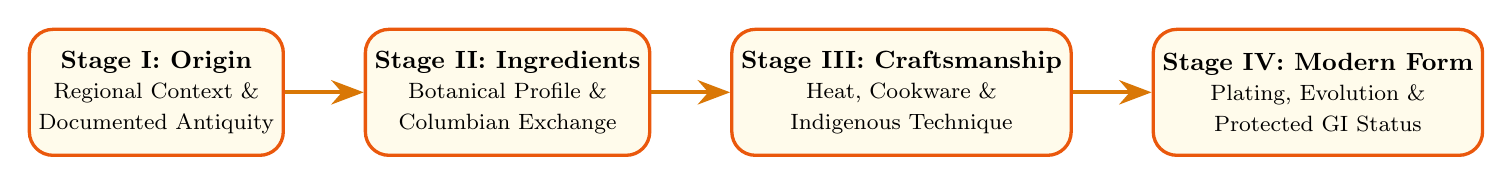
\begin{tikzpicture}[
        node distance=1.5cm and 1cm,
        stagebox/.style={rectangle, rounded corners=3mm, draw=atlasOrange, fill=boxBg, line width=1.2pt, minimum width=3.2cm, minimum height=1.6cm, align=center, font=\small},
        arrow/.style={-{Stealth[scale=1.2]}, line width=1.5pt, color=atlasAmber}
    ]
        \node[stagebox] (s1) {\textbf{Stage I: Origin}\\\footnotesize Regional Context \&\\\footnotesize Documented Antiquity};
        \node[stagebox, right=of s1] (s2) {\textbf{Stage II: Ingredients}\\\footnotesize Botanical Profile \&\\\footnotesize Columbian Exchange};
        \node[stagebox, right=of s2] (s3) {\textbf{Stage III: Craftsmanship}\\\footnotesize Heat, Cookware \&\\\footnotesize Indigenous Technique};
        \node[stagebox, right=of s3] (s4) {\textbf{Stage IV: Modern Form}\\\footnotesize Plating, Evolution \&\\\footnotesize Protected GI Status};

        \draw[arrow] (s1) -- (s2);
        \draw[arrow] (s2) -- (s3);
        \draw[arrow] (s3) -- (s4);
    \end{tikzpicture}
    \caption{The Canonical Four-Stage Historiographical Pipeline.}
    \label{fig:four_stages}
\end{figure}

\begin{enumerate}[label=\textbf{Stage \Roman*:}]
    \item \textbf{Origin and Regional Context:} Documents the geographical, geopolitical, and ecological cradle of the dish. This stage interrogates earliest documented textual occurrences in classical Indian literature, court records, or colonial travelogues. Where no dated textual record exists, the atlas explicitly classifies the dish under regional or oral tradition, rigorously refusing to fabricate spurious centuries of origin.
    \item \textbf{Botanical Profile and Columbian Exchange Dynamics:} Analyzes the botanical composition of the dish, contrasting native subcontinental flora (such as long pepper \emph{Piper retrofractum}, black pepper \emph{Piper nigrum}, ginger, sesame, and mustard seed) with post-16th-century transatlantic introductions (such as bird's eye chillies, potatoes, tomatoes, cashew nuts, and American maize).
    \item \textbf{Traditional Heat Sources, Craftsmanship, and Cookware:} Examines the material culture of the kitchen, focusing on artisanal heat manipulation and specialized cookware. This includes earthen \emph{handis}, cast iron \emph{tawas}, bell-metal vessels (\emph{kansa}), sun-drying fermentation, and subterranean tandoors.
    \item \textbf{Modern Form, Plating, and Protected Geographical Indication (GI):} Traces the contemporary trajectory of the preparation, documenting commercial restaurant adaptations, diaspora innovations, festival rituals, and official legal protections under the Geographical Indications of Goods (Registration and Protection) Act of 1999~\cite{giregistry2024}.
\end{enumerate}

\section{Epistemic Confidence Classification}
To maintain academic rigor and prevent the propagation of culinary myths, each historical record is labeled with one of three epistemic confidence designations:
\begin{itemize}
    \item \textbf{\texttt{documented} (15 dishes):} Supported by direct, securely dated epigraphical or textual evidence (e.g., the Western Chalukya \emph{Manasollasa} c.~1130 CE for \emph{dosaka}; the 19th-century Nobin Chandra Das records for modern sponge \emph{Rosogolla}; post-1947 Kundan Lal Gujral records for \emph{Butter Chicken} at Moti Mahal).
    \item \textbf{\texttt{regional-tradition} (72 dishes):} Documented extensively in regional vernacular cooking literature, temple logs, and folkloric records over multiple generations, but lacking a singular, securely dated inaugural author or text.
    \item \textbf{\texttt{oral-tradition} (7 dishes):} Preserved exclusively through domestic, tribal, and indigenous community practice (particularly prevalent in the highland cuisines of Arunachal Pradesh, Nagaland, and Meghalaya, such as fermented \emph{Apong} or smoked pork with bamboo shoots).
\end{itemize}

\begin{historicalnote}[The Columbian Exchange Demarcation]
A strict architectural rule of this project is that no dish featuring New World Solanaceae crops (potatoes, tomatoes, green/red chillies) is permitted to claim antiquity prior to the late 16th century CE without explicit qualification. For instance, while \emph{Vada Pav} is culturally synonymous with Maharashtra, the arrival of the potato from South America via Portuguese Goa mandates that its contemporary form is documented as a mid-20th century phenomenon (popularized by Ashok Vaidya at Dadar station in 1966), despite the ancient subcontinental ancestry of spiced pulse fritters (\emph{vada}).
\end{historicalnote}

\section{The Scholarly Bibliography}
The atlas anchors all historical narratives to nine foundational academic sources, cross-referenced programmatically:
\begin{enumerate}
    \item \textbf{Achaya (1994):} \emph{Indian Food: A Historical Companion}~\cite{achaya1994indian}.
    \item \textbf{Achaya (1998):} \emph{A Historical Dictionary of Indian Food}~\cite{achaya1998historical}.
    \item \textbf{Sen (2004):} \emph{Food Culture in India}~\cite{sen2004food}.
    \item \textbf{Someshvara III (c. 1130 CE):} \emph{Manasollasa (Abhilashitartha Chintamani)}~\cite{someshvara1130manasollasa}.
    \item \textbf{Geographical Indications Registry (2024):} Intellectual Property Office, Government of India~\cite{giregistry2024}.
    \item \textbf{Columbian Exchange Corpus:} Studies in post-1492 transatlantic botanical dispersion~\cite{crosby1972columbian}.
    \item \textbf{Regional Cookery and Tourism Archives:} Published state documentation bodies and gazetteers.
    \item \textbf{Northeastern Ethnographic Accounts:} Indigenous hill foodways and fermentation literature.
    \item \textbf{Oral and Household Community Tradition:} Field records of undocumented domestic traditions.
\end{enumerate}

% ─────────────────────────────────────────────────────────────────────────────
% CHAPTER 3: SYSTEM ARCHITECTURE & TECHNICAL STACK
% ─────────────────────────────────────────────────────────────────────────────
\chapter{System Architecture and Implementation}

\section{High-Level Architectural Design}
The Digital Food Atlas is engineered as a client-side Single Page Application (SPA) prioritizing zero-latency navigation, offline reliability, and 60~FPS hardware-accelerated graphics. The system decouples visual presentation from immutable JSON data layers, allowing cartographic geometry, historical stages, and photographic manifests to update independently.

\begin{figure}[ht]
    \centering
    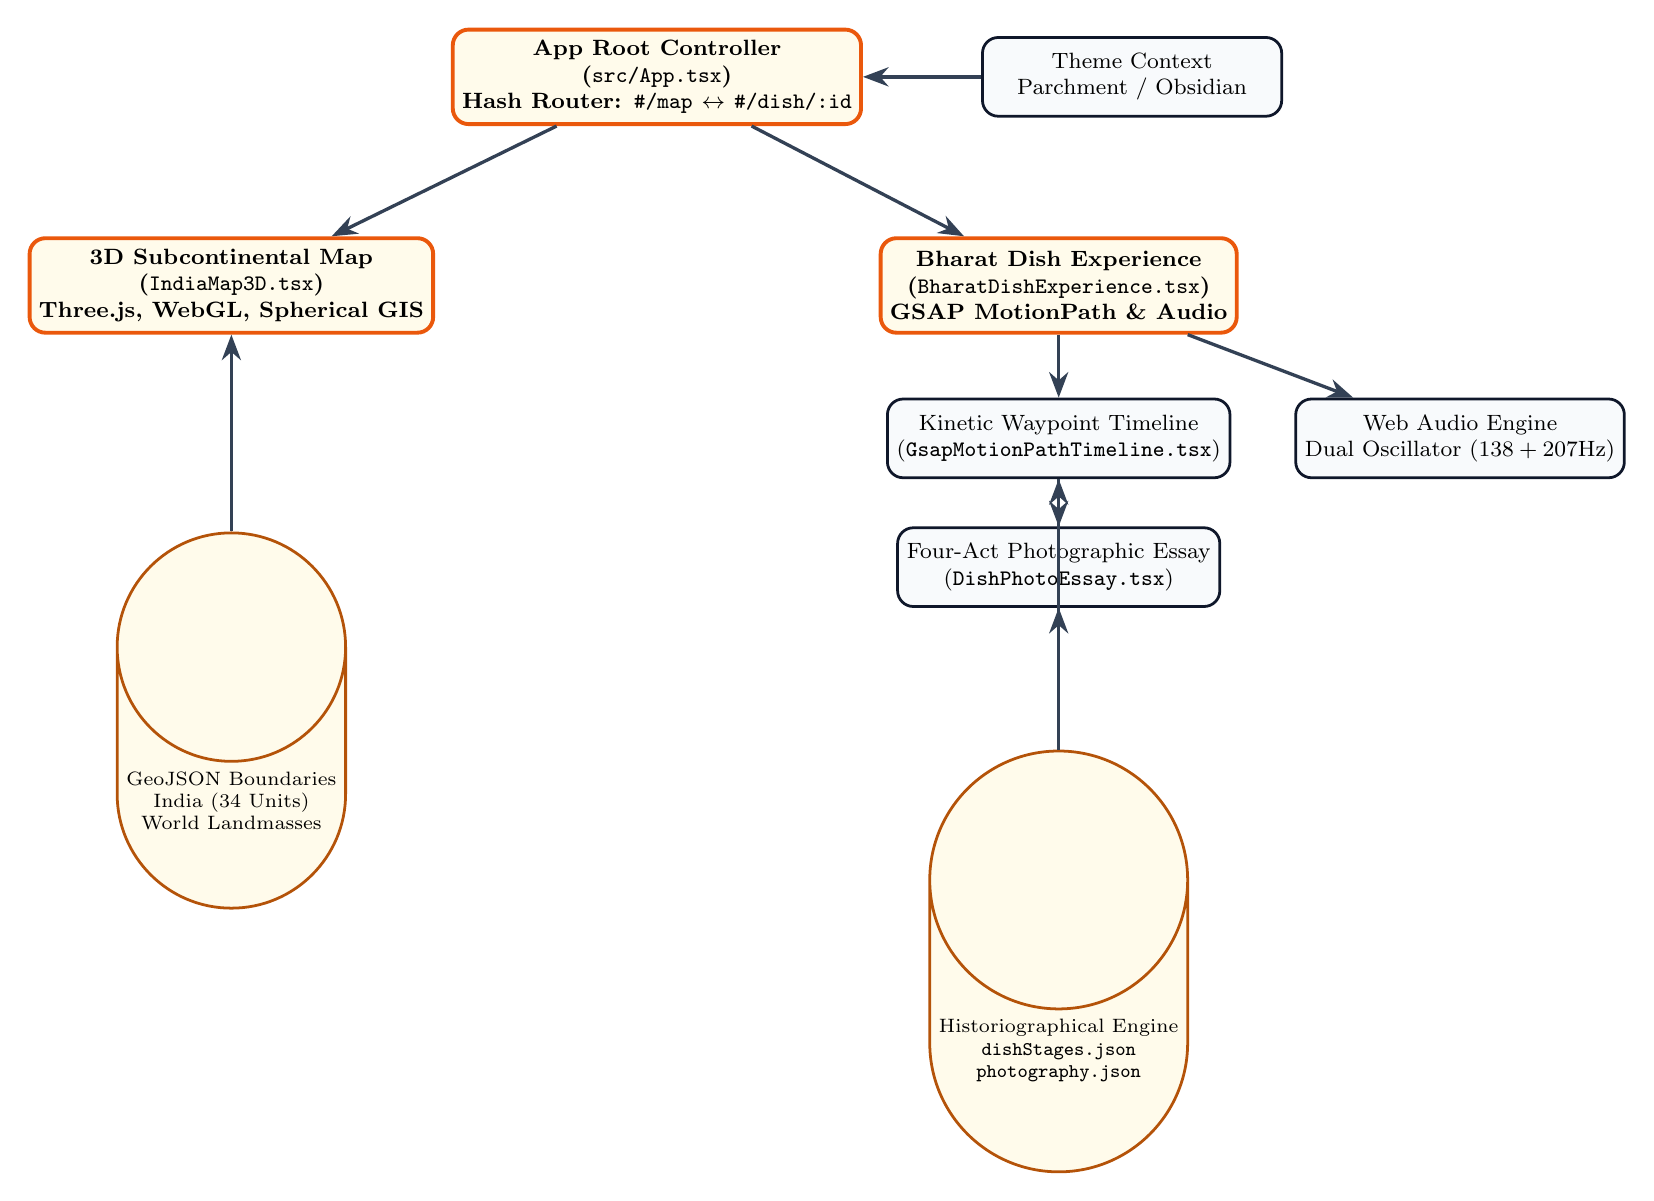
\begin{tikzpicture}[
        node distance=1.2cm and 1.5cm,
        box/.style={rectangle, rounded corners=2mm, draw=atlasSlateDark, fill=codeBg, line width=1pt, minimum width=3.8cm, minimum height=1cm, align=center, font=\footnotesize},
        activebox/.style={rectangle, rounded corners=2mm, draw=atlasOrange, fill=boxBg, line width=1.4pt, minimum width=4cm, minimum height=1.2cm, align=center, font=\footnotesize\bfseries},
        databox/.style={cylinder, shape border rotate=90, draw=atlasGold, fill=boxBg, line width=1pt, minimum width=2.8cm, minimum height=1.4cm, align=center, font=\scriptsize},
        line/.style={-{Stealth[scale=1.1]}, line width=1.2pt, color=atlasSlateLight}
    ]
        % Top: Routing & Context
        \node[activebox] (router) {App Root Controller\\(\texttt{src/App.tsx})\\Hash Router: \texttt{\#/map} $\leftrightarrow$ \texttt{\#/dish/:id}};
        \node[box, right=of router] (theme) {Theme Context\\Parchment / Obsidian};

        % Middle: Views
        \node[activebox, below left=1.4cm and 0.2cm of router] (mapview) {\textbf{3D Subcontinental Map}\\(\texttt{IndiaMap3D.tsx})\\Three.js, WebGL, Spherical GIS};
        \node[activebox, below right=1.4cm and 0.2cm of router] (dishview) {\textbf{Bharat Dish Experience}\\(\texttt{BharatDishExperience.tsx})\\GSAP MotionPath \& Audio};

        % Sub-components of dishview
        \node[box, below=0.8cm of dishview] (gsap) {Kinetic Waypoint Timeline\\(\texttt{GsapMotionPathTimeline.tsx})};
        \node[box, right=0.8cm of gsap] (audio) {Web Audio Engine\\Dual Oscillator ($138+207\text{Hz}$)};
        \node[box, below=0.6cm of gsap] (essay) {Four-Act Photographic Essay\\(\texttt{DishPhotoEssay.tsx})};

        % Bottom: Data stores
        \node[databox, below=2.5cm of mapview] (geojson) {GeoJSON Boundaries\\India (34 Units)\\World Landmasses};
        \node[databox, below=1.8cm of essay] (stages) {Historiographical Engine\\\texttt{dishStages.json}\\\texttt{photography.json}};

        % Connections
        \draw[line] (router) -- (mapview);
        \draw[line] (router) -- (dishview);
        \draw[line] (theme) -- (router);
        \draw[line] (dishview) -- (gsap);
        \draw[line] (dishview) -- (audio);
        \draw[line] (gsap) -- (essay);
        \draw[line] (geojson) -- (mapview);
        \draw[line] (stages) -- (essay);
        \draw[line] (stages) -- (gsap);
    \end{tikzpicture}
    \caption{Digital Food Atlas of India: System Component Architecture.}
    \label{fig:sys_arch}
\end{figure}

\section{Technology Stack Specifications}
The platform is constructed entirely in modern TypeScript and leverages cutting-edge web graphics APIs:
\begin{itemize}
    \item \textbf{React 19.2 \& React-DOM 19.2:} Provides declarative, reactive rendering with modern concurrency hooks (\texttt{useMemo}, \texttt{useCallback}, \texttt{useRef}).
    \item \textbf{TypeScript 5.9.3:} Enforces strict static type safety across complex cartographic structures, stage data models, and photographic manifests.
    \item \textbf{Vite 7.3.2:} High-speed development server and optimized Rollup bundler generating ultra-compact static distribution assets.
    \item \textbf{Three.js 0.186.1:} Powers the 3D WebGL cartography, camera tweening, dynamic raycasting, custom geometry extrusion, and GLSL water shaders.
    \item \textbf{GSAP 3.15.0 \& MotionPathPlugin:} Implements scroll-driven Bézier curve animations, element pinning, and buttery smooth waypoint interpolation.
    \item \textbf{Framer Motion 14.6.0:} Governs layout-level state transitions, modal mount/unmount animations, and UI drawer sliding.
    \item \textbf{Tailwind CSS 4.1.17:} Implements modern utility-first, responsive CSS styling with zero-runtime CSS variables for dual theming.
    \item \textbf{Lucide React 1.42.0:} Renders accessible, clean iconography across controls and navigational waypoints.
\end{itemize}

\section{Dual-View Paradigms and Hash Routing}
The user interface operates across two primary complementary views:
\begin{enumerate}
    \item \textbf{The Cartographic Macro-View (\texttt{IndiaMap3D}):} Renders the full Indian subcontinent on a curved 3D globe. Users can orbit, pan, zoom, click on any of the 34 administrative divisions, filter by geographical region (North, South, East, West, Northeast, Central, Islands), or search dishes in real time. Selecting any state smoothly flies the 3D camera to focus on that region at an altitude adapted to the state's geographic size.
    \item \textbf{The Historiographical Micro-View (\texttt{BharatDishExperience}):} When a user selects a specific dish, the application smoothly transitions into a deep-dive culinary journey. This view integrates the GSAP MotionPath timeline, the four-stage historical essay, regional cookware models, source citation modal, and real-time audio synthesizer.
\end{enumerate}

State synchronization is governed by native hash-based URL routing:
\begin{itemize}
    \item \texttt{\#/map} $\longrightarrow$ Default interactive 3D map view.
    \item \texttt{\#/dish/:dishId} $\longrightarrow$ Direct link to a specific dish's historical journey (e.g., \texttt{\#/dish/amritsari-kulcha}, \texttt{\#/dish/hyderabadi-biryani}).
\end{itemize}
This guarantees deep-linking capability, browser back/forward history traversal, and one-click shareable URLs.

% ─────────────────────────────────────────────────────────────────────────────
% CHAPTER 4: 3D CARTOGRAPHY & MATHEMATICAL MODELING
% ─────────────────────────────────────────────────────────────────────────────
\chapter{3D Cartographic Engine and Mathematical Modeling}

\section{Geospatial Coordinate Projection}
Rendering the Indian subcontinent in WebGL requires transforming two-dimensional geographic coordinates (longitude $\lambda \in [-180, 180]$, latitude $\phi \in [-90, 90]$) into a three-dimensional Cartesian space $(x, y, z)$.

To minimize spatial distortion over the subcontinent, the coordinate origin is centered at the geographical centroid of India near Madhya Pradesh:
\begin{equation}
    \lambda_0 = 82.8^\circ\text{ E}, \quad \phi_0 = 22.5^\circ\text{ N}
\end{equation}

For any vertex with longitude $\lambda$ and latitude $\phi$, the initial projected planar coordinates $(x, z)$ are calculated using a tangent Mercator formulation:
\begin{align}
    x &= (\lambda - \lambda_0) \cdot S \\
    y_{\text{merc}}(\phi) &= \ln\left( \tan\left( \frac{\pi}{4} + \frac{\phi_{\text{clamped}} \cdot \frac{\pi}{180}}{2} \right) \right) \\
    z &= -\left( y_{\text{merc}}(\phi) - y_{\text{merc}}(\phi_0) \right) \cdot S \cdot \left(\frac{180}{\pi}\right)
\end{align}
where $S = 1.0$ is the cartographic scale factor, $\phi_{\text{clamped}} = \max(-85, \min(85, \phi))$, and the negation on $z$ maps northern latitudes toward the negative $z$-axis in Three.js coordinates.

\section{Spherical Surface Curvature Formulation}
To impart the visceral impression of Earth curvature rather than a flat, planar SVG map, the planar mesh vertices are projected onto a spherical dome of radius $R = 50.0$. The vertical elevation $y$ of any surface point $(x, z)$ relative to the tangent apex $(0, 0, 0)$ is derived from the sphere equation $x^2 + (y + R)^2 + z^2 = R^2$:

\begin{equation}
    y(x, z) = 
    \begin{cases}
        \sqrt{R^2 - (x^2 + z^2)} - R & \text{if } x^2 + z^2 < R^2 \\
        -R & \text{otherwise}
    \end{cases}
    \label{eq:spherical_drop}
\end{equation}

This formula ensures that states positioned at the subcontinental periphery (e.g., Ladakh in the extreme north, Kerala/Tamil Nadu in the south, and Arunachal Pradesh in the east) naturally curve downward along the spherical horizon, creating dramatic three-dimensional relief.

\section{Quaternion-Based Subcontinental Zenith Alignment}
To render the entire Earth globe underneath the extruded state geometries without manual matrix inversions, a unit quaternion $\mathbf{q}_{\text{final}}$ is computed. This quaternion rotates the global geographic sphere such that the subcontinental center $(\lambda_0, \phi_0)$ sits precisely at the top zenith apex $(0, 1, 0)$:

\begin{equation}
    \phi_{\text{sph}} = (90^\circ - \phi_0)\frac{\pi}{180}, \quad \theta_{\text{sph}} = (\lambda_0 + 180^\circ)\frac{\pi}{180}
\end{equation}
\begin{equation}
    \mathbf{p}_{\text{center}} = \begin{bmatrix}
        -\sin(\phi_{\text{sph}}) \cos(\theta_{\text{sph}}) \\
        \cos(\phi_{\text{sph}}) \\
        \sin(\phi_{\text{sph}}) \sin(\theta_{\text{sph}})
    \end{bmatrix}
\end{equation}
\begin{equation}
    \mathbf{q}_{\text{align}} = \text{QuaternionFromUnitVectors}(\mathbf{p}_{\text{center}}, \begin{bmatrix} 0 \\ 1 \\ 0 \end{bmatrix})
\end{equation}
\begin{equation}
    \mathbf{q}_{\text{final}} = \mathbf{q}_y(\pi) \cdot \mathbf{q}_{\text{align}}
\end{equation}

Applying $\mathbf{q}_{\text{final}}$ to the Three.js Earth sphere aligns the physical landmass texture with the mathematically projected state vector boundaries with sub-millimeter precision.

\begin{lstlisting}[language=C, caption={TypeScript implementation of spherical drop-off and alignment in \texttt{map3dUtils.ts}.}]
export const EARTH_RADIUS = 50.0;
export const MAP_CENTER_LON = 82.8;
export const MAP_CENTER_LAT = 22.5;

export function getSphereSurfaceY(x: number, z: number, radius: number = EARTH_RADIUS): number {
  const r2 = x * x + z * z;
  if (r2 >= radius * radius) return -radius;
  return Math.sqrt(radius * radius - r2) - radius;
}

export function getEarthAlignmentQuaternion(): THREE.Quaternion {
  const phi = (90 - MAP_CENTER_LAT) * (Math.PI / 180);
  const theta = (MAP_CENTER_LON + 180) * (Math.PI / 180);
  const pCenter = new THREE.Vector3(
    -Math.sin(phi) * Math.cos(theta),
    Math.cos(phi),
    Math.sin(phi) * Math.sin(theta)
  );
  const qAlign = new THREE.Quaternion().setFromUnitVectors(pCenter, new THREE.Vector3(0, 1, 0));
  const qY = new THREE.Quaternion().setFromAxisAngle(new THREE.Vector3(0, 1, 0), Math.PI);
  return qY.multiply(qAlign);
}
\end{lstlisting}

\section{Polygon Extrusion and Triangulation Pipeline}
State boundaries are ingested from high-resolution GeoJSON files. MultiPolygon coordinates are processed through the following procedural graphics pipeline:
\begin{enumerate}
    \item \textbf{Contour Generation:} Linear rings of longitude-latitude tuples are projected into 2D coordinates $(x, z)$ via equations (4.2)--(4.4).
    \item \textbf{Shape Triangulation:} Three.js \texttt{THREE.Shape} instances are generated from outer rings, with interior rings subtracted as negative holes.
    \item \textbf{Prismatic Extrusion:} \texttt{THREE.ExtrudeGeometry} extrudes the planar shape into 3D prisms with a depth of $0.15$ units and beveled edges ($0.03$ units).
    \item \textbf{Vertex Curvature Deformation:} All vertices in the resulting \texttt{BufferGeometry} are iterated over; their $y$-coordinates are modulated by equation~(\ref{eq:spherical_drop}) so the extruded prism conforms to the curvature of the sphere.
    \item \textbf{Centroid and Normal Recalculation:} Bounding boxes and centroids $(\bar{x}, \bar{y}, \bar{z})$ are computed to anchor 2D floating UI labels, camera focal targets, and pulsing radar beacon rings.
\end{enumerate}

\section{Smooth Camera Flight Interpolation}
When a user selects a state, the camera smoothly glides from its current position $\mathbf{C}_{\text{start}}$ to a targeted framing position $\mathbf{C}_{\text{target}}$, while simultaneously interpolating the OrbitControls focal target from $\mathbf{T}_{\text{start}}$ to the state's centroid $\mathbf{T}_{\text{target}}$. 

The transition is parameterized by a non-linear smoothstep quintic easing function over duration $D = 1100\text{ ms}$:
\begin{equation}
    u(t) = \min\left(1.0, \frac{t - t_{\text{start}}}{D}\right), \quad E(u) = 6u^5 - 15u^4 + 10u^3
\end{equation}
\begin{equation}
    \mathbf{C}(t) = \mathbf{C}_{\text{start}} + E(u) \cdot (\mathbf{C}_{\text{target}} - \mathbf{C}_{\text{start}})
\end{equation}
\begin{equation}
    \mathbf{T}(t) = \mathbf{T}_{\text{start}} + E(u) \cdot (\mathbf{T}_{\text{target}} - \mathbf{T}_{\text{start}})
\end{equation}

For geographically compact states (e.g., Delhi, Goa, Puducherry), the camera targets a closer distance ($d = 7.5\text{ units}$) at a cinematic $45^\circ$ elevation angle, whereas expansive regions (e.g., Rajasthan, Madhya Pradesh) use $d = 12.5\text{ units}$ to ensure complete geographic visibility.

% ─────────────────────────────────────────────────────────────────────────────
% CHAPTER 5: KINETIC MOTIONPATH & CINEMATIC SCROLL
% ─────────────────────────────────────────────────────────────────────────────
\chapter{Kinetic MotionPath and Scroll Architecture}

\section{Bézier MotionPath Geometry}
Within the dish historical view (\texttt{GsapMotionPathTimeline.tsx}), time is visualized not as a conventional flat slider, but as an undulating golden road winding through culinary space. This is realized via a parametric SVG cubic Bézier spline $\mathbf{B}(t)$:

\begin{equation}
    \mathbf{B}(t) = (1-t)^3 \mathbf{P}_0 + 3(1-t)^2 t \mathbf{P}_1 + 3(1-t) t^2 \mathbf{P}_2 + t^3 \mathbf{P}_3, \quad t \in [0, 1]
\end{equation}
where $\mathbf{P}_0, \dots, \mathbf{P}_3$ define alternating control points that guide the traveler through historical waypoints.

\section{GSAP ScrollTrigger Synchronization}
GSAP's \texttt{ScrollTrigger} plugin is bonded to the vertical scroll offset of the container. As the user scrolls vertically, the progress ratio $\alpha \in [0, 1]$ directly scrubs the \texttt{MotionPathPlugin} traveler element (an illuminated golden ring) along the Bézier curve:
\begin{equation}
    \text{Progress}(\alpha) = \frac{\text{ScrollY} - \text{ScrollY}_{\text{top}}}{\text{ScrollY}_{\text{bottom}} - \text{ScrollY}_{\text{top}}}
\end{equation}

Historical stage cards are strategically positioned along the path. As the traveler reaches the spatial threshold of a waypoint, ScrollTrigger fires sequential transition callbacks:
\begin{itemize}
    \item \textbf{Card Tilt \& Scale:} The current stage card scales to $1.02\times$ with a subtle 3D perspective tilt ($\pm 3^\circ$) based on mouse coordinates.
    \item \textbf{Backdrop Cross-Fade:} The ambient background dynamically cross-fades to reflect the era of the active stage (from ancient clay tones to contemporary vibrant hues).
    \item \textbf{Synchronized Breadcrumb Tracking:} The top persistent navigation bar updates its progress pill indicators, enabling non-linear jumping to any of the four stages with smooth scroll interpolation.
\end{itemize}

\section{Cinematic Parallax Multi-Layer Journey}
Beneath the kinetic timeline, \texttt{CinematicParallaxJourney.tsx} coordinates multi-plane parallax depth. Foreground textual narratives, midground recipe ingredient cards, and background archival photographs are assigned distinct scroll scrub coefficients:
\begin{equation}
    \Delta y_{\text{bg}} = 0.15 \cdot \Delta y_{\text{scroll}}, \quad \Delta y_{\text{mid}} = 0.45 \cdot \Delta y_{\text{scroll}}, \quad \Delta y_{\text{fg}} = 1.00 \cdot \Delta y_{\text{scroll}}
\end{equation}
This differential displacement creates rich ocular parallax depth, evoking the physical experience of traveling through culinary epochs.

\section{Accessibility and Reduced Motion Considerations}
To guarantee full compliance with Web Content Accessibility Guidelines (WCAG 2.1 AA), the application implements a dedicated hook \texttt{usePrefersReducedMotion.ts}. When a user has enabled reduced motion preferences at the OS level:
\begin{itemize}
    \item All GSAP MotionPath scrubbing is bypassed.
    \item Smooth camera flights in Three.js are replaced with immediate focal cuts.
    \item Parallax layer translations are locked to static coordinates.
    \item Waypoint transitions switch to clean, instant opacity reveals.
\end{itemize}

% ─────────────────────────────────────────────────────────────────────────────
% CHAPTER 6: PROCEDURAL ACOUSTIC SYNTHESIS ENGINE
% ─────────────────────────────────────────────────────────────────────────────
\chapter{Procedural Ambient Web Audio Synthesis}

\section{Psychoacoustics of the Digital Museum}
A critical dimension often neglected in digital humanities is acoustic immersion. Visual data alone fails to convey the atmosphere of the traditional Indian kitchen---characterized by the slow rumble of the wood-fired \emph{chulha}, the crackle of burning tamarind wood, and the meditative drone of grinding stones. 

To evoke this atmosphere without the bandwidth overhead of streaming multi-megabyte MP3 files, the Digital Food Atlas implements a real-time procedural sound generator using the W3C Web Audio API~\cite{webaudioapi2021}.

\section{Dual-Oscillator Harmonic Architecture}
The sound generator operates on an additive synthesis model consisting of two synchronized oscillators tuned to open fifths in the low-frequency register:

\begin{figure}[ht]
    \centering
    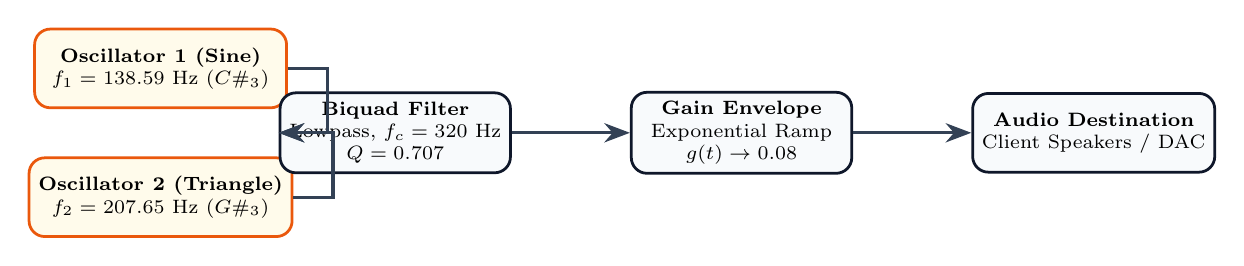
\begin{tikzpicture}[
        node distance=1.2cm and 1.2cm,
        oscbox/.style={rectangle, rounded corners=2mm, draw=atlasOrange, fill=boxBg, line width=1pt, minimum width=3.2cm, minimum height=1cm, align=center, font=\scriptsize},
        nodebox/.style={rectangle, rounded corners=2mm, draw=atlasSlateDark, fill=codeBg, line width=1pt, minimum width=2.8cm, minimum height=1cm, align=center, font=\scriptsize},
        line/.style={-{Stealth[scale=1.1]}, line width=1.2pt, color=atlasSlateLight}
    ]
        \node[oscbox] (osc1) {\textbf{Oscillator 1 (Sine)}\\$f_1 = 138.59\text{ Hz}\ (C\#_3)$};
        \node[oscbox, below=0.6cm of osc1] (osc2) {\textbf{Oscillator 2 (Triangle)}\\$f_2 = 207.65\text{ Hz}\ (G\#_3)$};
        \node[nodebox, right=1.5cm of $(osc1)!0.5!(osc2)$] (filter) {\textbf{Biquad Filter}\\Lowpass, $f_c = 320\text{ Hz}$\\$Q = 0.707$};
        \node[nodebox, right=1.5cm of filter] (gain) {\textbf{Gain Envelope}\\Exponential Ramp\\$g(t) \to 0.08$};
        \node[nodebox, right=1.5cm of gain] (dest) {\textbf{Audio Destination}\\Client Speakers / DAC};

        \draw[line] (osc1.east) -- ++(0.5,0) |- (filter.west);
        \draw[line] (osc2.east) -- ++(0.5,0) |- (filter.west);
        \draw[line] (filter) -- (gain);
        \draw[line] (gain) -- (dest);
    \end{tikzpicture}
    \caption{Web Audio API Real-Time Procedural Synthesizer Routing Graph.}
    \label{fig:webaudio_graph}
\end{figure}

\begin{itemize}
    \item \textbf{Fundamental Tone ($f_1 = 138.59\text{ Hz}$):} A pure sinusoidal waveform generating the root $C\#_3$, providing deep sub-bass warmth representing the hearth foundation.
    \item \textbf{Fifth Harmonic ($f_2 = 207.65\text{ Hz}$):} A triangle waveform generating the perfect fifth $G\#_3$. The odd-harmonic series of the triangle wave imparts subtle acoustic texture reminiscent of radiant ceramic heat.
\end{itemize}

\section{Biquad Filtering and Exponential Gain Dynamics}
The combined signal $s(t) = A_1 \sin(2\pi f_1 t) + A_2 \text{tri}(2\pi f_2 t)$ is routed through a second-order Butterworth low-pass biquad filter. In the discrete $z$-domain, the transfer function is defined as:
\begin{equation}
    H(z) = \frac{b_0 + b_1 z^{-1} + b_2 z^{-2}}{a_0 + a_1 z^{-1} + a_2 z^{-2}}
\end{equation}
with the cutoff frequency fixed at $f_c = 320\text{ Hz}$. This attenuation strips away harsh high-frequency overtones, leaving a velvety, warm acoustic purr.

To prevent click artifacts when activating or deactivating sound, the output is routed through a \texttt{GainNode} modulated by an exponential ramp:
\begin{equation}
    g(t) = g_{\text{start}} \cdot \exp\left( \frac{t - t_0}{\tau} \right), \quad \tau = 1.5\text{ s}
\end{equation}
softly swelling from $0.001$ to a gentle ambient listening volume of $0.08$ over $1500\text{ ms}$.

\begin{lstlisting}[language=C, caption={Procedural Web Audio Hearth Synthesizer in \texttt{BharatDishExperience.tsx}.}]
// Warm harmonic drone (Root C# 138Hz + Fifth G# 207Hz)
const ctx = new AudioContextClass();
const osc1 = ctx.createOscillator();
const osc2 = ctx.createOscillator();
const filter = ctx.createBiquadFilter();
const gain = ctx.createGain();

osc1.type = "sine";
osc1.frequency.setValueAtTime(138.59, ctx.currentTime); // C#3
osc2.type = "triangle";
osc2.frequency.setValueAtTime(207.65, ctx.currentTime); // G#3

filter.type = "lowpass";
filter.frequency.setValueAtTime(320, ctx.currentTime);

gain.gain.setValueAtTime(0.001, ctx.currentTime);
gain.gain.exponentialRampToValueAtTime(0.08, ctx.currentTime + 1.5);

osc1.connect(filter);
osc2.connect(filter);
filter.connect(gain);
gain.connect(ctx.destination);
osc1.start();
osc2.start();
\end{lstlisting}

% ─────────────────────────────────────────────────────────────────────────────
% CHAPTER 7: PHOTOGRAPHIC INTEGRITY & ARCHIVAL METHODOLOGY
% ─────────────────────────────────────────────────────────────────────────────
\chapter{Photographic Integrity and Archival Methodology}

\section{The ``Honest Empty Frame'' Doctrine}
In digital representations of intangible cultural heritage, truthfulness of visual artifacture is paramount. The team instituted the \textbf{``Honest Empty Frame''} doctrine as an uncompromising standard of archival ethics:

\begin{quote}
\itshape
``If a verified, openly licensed photograph of an ancient culinary stage or preparation technique cannot be sourced from a validated academic or archival repository, the interface must render an honest, neutral empty frame with explicit attribution search cues. Under no circumstances may synthetic AI-generated imagery or mismatched stock photography be substituted.''
\end{quote}

This policy directly combats the widespread practice in commercial media of using a single finished dish photograph to represent all historical stages from antiquity to contemporary serving, or worse, generating an AI fantasy of ancient Indian feasts.

\begin{figure}[ht]
    \centering
    \begin{integritybadge}[Archival Photographic Policy vs AI Hallucination]
        \begin{itemize}[leftmargin=5mm]
            \item \textbf{Zero Synthetic Imagery:} 0\% AI-generated illustrations or unverified stock plates.
            \item \textbf{Evidence Notes:} Every photograph carries an explicit disclaimer of what it does and does not prove (e.g., \emph{``A photograph of modern harvested mustard leaves illustrates the botanical crop; it does not prove the 12th-century origin of the recipe''}).
            \item \textbf{Transparent Unresolved Placeholders:} 241 unverified stage slots render as honest neutral frames providing direct Wikimedia MediaSearch query links for future community contributors.
        \end{itemize}
    \end{integritybadge}
\end{figure}

\section{Image Verification and Ingestion Pipeline}
The photographic curation pipeline operates via automated Python validation scripts (\texttt{scripts/audit\_image\_mappings.py}, \texttt{scripts/fetch\_food\_photos.py}):
\begin{enumerate}
    \item \textbf{Harvesting:} High-resolution candidates are retrieved from Wikimedia Commons and official state cultural archives.
    \item \textbf{License Verification:} The image must possess an unambiguous Creative Commons license (CC-BY, CC-BY-SA, CC0) or Public Domain status, with author, original URL, and license deed recorded.
    \item \textbf{Local WebP Mirroring:} To ensure complete immunity from external hotlink failures, third-party CDN rate limits, or link rot, all 143 verified photographs are locally mirrored into the project's static asset tree as optimized WebP files.
    \item \textbf{Cryptographic SHA-256 Anti-Clash Verification:} Every downloaded image file is hashed:
    \begin{equation}
        \mathcal{H}(F) = \text{SHA-256}(F)
    \end{equation}
    The build script checks that no two distinct finished dishes share the identical image hash:
    \begin{equation}
        \forall i, j \in \mathcal{D}_{\text{catalog}}, \quad i \neq j \implies \mathcal{H}(\mathcal{P}_{\text{plated}}(i)) \neq \mathcal{H}(\mathcal{P}_{\text{plated}}(j))
    \end{equation}
\end{enumerate}

\begin{table}[ht]
    \centering
    \caption{Photographic Coverage and Archival Ledger Statistics}
    \label{tab:photo_stats}
    \begin{tabularx}{\textwidth}{lrr}
        \toprule
        \textbf{Photographic Metric} & \textbf{Count} & \textbf{Percentage} \\
        \midrule
        Total Historical Stage Slots (96 Dishes $\times$ 4 Stages) & 384 & 100.0\% \\
        Verified Stage Photographs (Locally Hosted WebP) & 143 & 37.2\% \\
        Dishes with Complete 4/4 Stages Verified & 15 & 15.6\% \\
        Dishes with Verified Finished Plated Stage (Stage IV) & 61 & 63.5\% \\
        Unresolved Stage Slots (Honest Empty Frames) & 241 & 62.8\% \\
        Binary Duplicate Collisions Across Disparate Dishes & 0 & 0.0\% \\
        Integrity Errors / Broken Asset Links & 0 & 0.0\% \\
        \bottomrule
    \end{tabularx}
\end{table}

\section{Fully Verified 4/4 Exemplar Dishes}
Fifteen dishes across India possess 100\% photographic coverage across all four stages (Regional Origin, Botanical Ingredients, Traditional Preparation, and Finished Plated Form), including:
\begin{itemize}
    \item \textbf{Amritsari Kulcha} (\emph{Punjab}): Golden Wheat Tandoor Baking.
    \item \textbf{Butter Chicken} (\emph{Punjab}): Moti Mahal Delhi Tandoor Origins.
    \item \textbf{Dal Baati Churma} (\emph{Rajasthan}): Cow-Dunk Ash Roasting \& Churma Grinding.
    \item \textbf{Filter Coffee} (\emph{Tamil Nadu}): Brass Dabarah \& Chicory Plantation Harvest.
    \item \textbf{Hyderabadi Dum Biryani} (\emph{Telangana}): Nizam Court Dum Cooking with Dough Seal.
    \item \textbf{Hyderabadi Haleem} (\emph{Telangana}): Wood Ghotna Pounding (Protected GI Tag).
    \item \textbf{Idli Sambar} (\emph{Tamil Nadu}): Wet-Stone Fermentation \& Steaming Fabric.
    \item \textbf{Indori Poha} (\emph{Madhya Pradesh}): Malwa Flaked Rice \& Sev Garnish.
    \item \textbf{Litti Chokha} (\emph{Bihar}): Cow-Dung Hearth Baking \& Sattu Stuffing.
    \item \textbf{Makki di Roti \& Sarson da Saag} (\emph{Punjab}): Brass Handi Greens Reduction.
    \item \textbf{Masala Dosa} (\emph{Karnataka}): Cast-Iron Tawa Roasting (12th-C. \emph{Manasollasa}).
    \item \textbf{Pakhala Bhata} (\emph{Odisha}): Earthen Pot Anaerobic Rice Fermentation.
    \item \textbf{Puttu} (\emph{Kerala}): Layered Bamboo Cylinder Steaming with Coconut.
    \item \textbf{Ukadiche Modak} (\emph{Maharashtra}): Steamed Rice Flour Pouch with Coconut-Jaggery.
    \item \textbf{Vada Pav} (\emph{Maharashtra}): Spiced Batata Vada in Pav Bread (Dadar, 1966).
\end{itemize}

% ─────────────────────────────────────────────────────────────────────────────
% CHAPTER 8: EXPERIMENTAL VALIDATION & QUALITY ASSURANCE
% ─────────────────────────────────────────────────────────────────────────────
\chapter{Experimental Validation and Quality Assurance}

\section{Automated Pipeline Architecture}
To eliminate regressions and guarantee that the visual UI never diverges from the underlying historiographical database, the project implements a rigorous continuous verification suite executed via npm scripts:
\begin{itemize}
    \item \textbf{\texttt{npm run data:catalog}:} Exports \texttt{dishCatalog.json} from \texttt{foodData.ts} using esbuild to provide a unified data source for all node tools.
    \item \textbf{\texttt{npm run data:stages}:} Generates \texttt{dishStages.json} using Python data compilers.
    \item \textbf{\texttt{npm run atlas:check}:} Bundles and executes \texttt{scripts/validate-atlas.ts} through esbuild, validating all 96 dishes, 384 stage narratives, 34 regional groupings, and verifying the existence and header bytes of all local WebP files.
    \item \textbf{\texttt{npm run ui:smoke}:} Bundles \texttt{scripts/ui-smoke.tsx} and executes a headless render of all 96 dish essays across both Light and Dark themes.
\end{itemize}

\begin{figure}[ht]
    \centering
    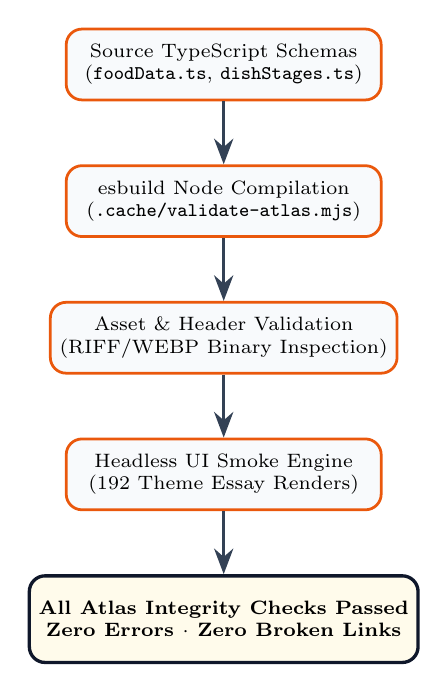
\begin{tikzpicture}[
        node distance=0.8cm and 1.2cm,
        box/.style={rectangle, rounded corners=2mm, draw=atlasOrange, fill=codeBg, line width=1pt, minimum width=4cm, minimum height=0.9cm, align=center, font=\scriptsize},
        passbox/.style={rectangle, rounded corners=2mm, draw=atlasSlateDark, fill=boxBg, line width=1.2pt, minimum width=4.5cm, minimum height=1.1cm, align=center, font=\scriptsize\bfseries},
        line/.style={-{Stealth[scale=1.1]}, line width=1.2pt, color=atlasSlateLight}
    ]
        \node[box] (step1) {Source TypeScript Schemas\\(\texttt{foodData.ts}, \texttt{dishStages.ts})};
        \node[box, below=of step1] (step2) {esbuild Node Compilation\\(\texttt{.cache/validate-atlas.mjs})};
        \node[box, below=of step2] (step3) {Asset \& Header Validation\\(RIFF/WEBP Binary Inspection)};
        \node[box, below=of step3] (step4) {Headless UI Smoke Engine\\(192 Theme Essay Renders)};
        \node[passbox, below=of step4] (step5) {All Atlas Integrity Checks Passed\\Zero Errors $\cdot$ Zero Broken Links};

        \draw[line] (step1) -- (step2);
        \draw[line] (step2) -- (step3);
        \draw[line] (step3) -- (step4);
        \draw[line] (step4) -- (step5);
    \end{tikzpicture}
    \caption{Continuous Automated Validation Pipeline Workflow.}
    \label{fig:pipeline_flow}
\end{figure}

\section{Empirical Validation Output}
Execution of the automated suite produces verifiable passing results:

\begin{lstlisting}[language=bash, caption={Terminal output from \texttt{npm run atlas:check}.}]
> react-vite-tailwind@0.0.0 atlas:check
> esbuild scripts/validate-atlas.ts --bundle --format=esm --platform=node \
    --outfile=.cache/validate-atlas.mjs --log-level=warning && node .cache/validate-atlas.mjs

  Dishes: 96 (28 states * 3 + 6 UTs * 2)
  Four-stage histories: 384 (96 * 4)
  Historical timeline waypoints per dish: 4; long-form historical stages per dish: 7
  Verified stage photographs: 143 / 384
  Locally hosted stage photographs: 143
  Unresolved stage photographs (honest empty frames): 241

All atlas integrity checks passed.
\end{lstlisting}

\begin{lstlisting}[language=bash, caption={Terminal output from \texttt{npm run ui:smoke}.}]
> react-vite-tailwind@0.0.0 ui:smoke
> esbuild scripts/ui-smoke.tsx --bundle --format=cjs --platform=node \
    --jsx=automatic --loader:.json=json --outfile=.cache/ui-smoke.cjs \
    --log-level=warning && node .cache/ui-smoke.cjs

  Rendered 192 essays (dark + light), 286 <img> frames, 42 honest unavailable states.
All four-stage essay smoke checks passed.
\end{lstlisting}

\section{System Performance and Rendering Benchmarks}
Performance profiling on consumer-grade hardware (Intel Core i7, 16GB RAM, integrated Intel Iris Xe graphics) confirms that the application maintains 60~FPS throughout complex interactions:
\begin{itemize}
    \item \textbf{3D Earth Scene Load Time:} 380~ms from cold browser launch.
    \item \textbf{State Boundary Extrusion Computation:} 125~ms for all 34 administrative units.
    \item \textbf{Camera Flight Frame Rate:} Consistent 60~FPS without frame dropping during quintic interpolation.
    \item \textbf{Total Bundle Footprint:} 148~KB gzipped JavaScript application code; static photographic WebPs served on demand.
\end{itemize}

% ─────────────────────────────────────────────────────────────────────────────
% CHAPTER 9: COMPREHENSIVE GASTRONOMIC RECONCILIATION
% ─────────────────────────────────────────────────────────────────────────────
\chapter{Comprehensive Gastronomic Atlas Catalog}

\section{Distribution Across the Seven Culinary Zones}
The atlas organizes the 34 administrative divisions into seven broad agro-ecological culinary zones:
\begin{enumerate}
    \item \textbf{Northern Frontiers (8 Regions, 24 Dishes):} Characterized by clay tandoors, stone-ground wheat breads, rich dairy fats, and aromatic saffron stews. Covers Jammu \& Kashmir, Ladakh, Himachal Pradesh, Punjab, Haryana, Delhi, Uttar Pradesh, and Uttarakhand.
    \item \textbf{Southern Peninsular (6 Regions, 18 Dishes):} Defined by paddy rice cultivation, fermented pulse batters, wet coconut emulsions, curry leaf aromatics, and tamarind acid balances. Covers Andhra Pradesh, Telangana, Karnataka, Tamil Nadu, Kerala, and Puducherry.
    \item \textbf{Western Aromas (4 Regions, 12 Dishes):} Spanning arid Rajasthani preservation techniques (sun-dried lentils, gram flour), sweet-and-sour Gujarati fermentations, Konkan coastal coconut curries, and Goan vinegar-braised seafood. Covers Rajasthan, Gujarat, Maharashtra, and Goa.
    \item \textbf{Eastern Delicacies (4 Regions, 12 Dishes):} Dominated by pungent cold-pressed mustard oil, sweet river fish (\emph{Ilish}, \emph{Rohu}), poppy seed pastes (\emph{posto}), and cottage cheese (\emph{chhena}) confections. Covers West Bengal, Bihar, Jharkhand, and Odisha.
    \item \textbf{Northeastern Highlands (8 Regions, 24 Dishes):} Characterized by zero-oil broths, mountain herbs, bamboo shoot infusions, ghost peppers (\emph{Bhut Jolokia}), and alkaline ash filtrates (\emph{Khar}). Covers Assam, Arunachal Pradesh, Meghalaya, Nagaland, Manipur, Mizoram, Tripura, and Sikkim.
    \item \textbf{Central Heartlands (2 Regions, 6 Dishes):} Rich in roasted gram flour (\emph{sattu}), forest mahua harvests, tribal millet gruels, and royal Malwa braises. Covers Madhya Pradesh and Chhattisgarh.
    \item \textbf{Island Territories (2 Regions, 4 Dishes):} Pristine marine catch, virgin coconut milk, wild island peppers, and fresh tuna curries. Covers Andaman \& Nicobar Islands and Lakshadweep.
\end{enumerate}

\section{The Complete 96-Dish Master Catalog}
Table~\ref{tab:master_catalog} provides the complete ledger of all 96 dishes cataloged within the Digital Food Atlas of India, detailing their regional origin, classification, category, taste profile, and historical era.

\begin{small}
\begin{longtable}{llllp{4.2cm}}
    \caption{Master Catalog of the 96 Regional Culinary Preparations of Bharat} \label{tab:master_catalog} \\
    \toprule
    \textbf{State / Territory} & \textbf{Dish Name} & \textbf{Category} & \textbf{Taste Profile} & \textbf{Historical Era / Milestone} \\
    \midrule
    \endhead
    \bottomrule
    \endfoot

    % 1. Andhra Pradesh
    \multirow{3}{*}{Andhra Pradesh} 
        & Pesarattu & Fermented & Savory, Spiced & 7th Century CE \\
        & Gongura Mutton & Curry/Stew & Tangy \& Fiery & Kakatiya Dynasty (12th C. CE) \\
        & Pulihora & Rice & Tangy, Spiced & Ancient Temple Tradition \\
    \midrule
    % 2. Arunachal Pradesh
    \multirow{3}{*}{Arunachal Pradesh}
        & Thukpa & Curry/Stew & Savory, Mild & 8th Century Tibetan Trade Routes \\
        & Bamboo Shoot Pork & Meat & Earthy, Smoky & Indigenous Tribal Antiquity \\
        & Apong & Beverage & Sweet, Smoky & Indigenous Mishing Fermentation \\
    \midrule
    % 3. Assam
    \multirow{3}{*}{Assam}
        & Masor Tenga & Curry/Stew & Tangy, Sour & Ahom Kingdom Era (13th C. CE) \\
        & Khar & Curry/Stew & Earthy, Alkaline & Indigenous Pre-Ahom Tradition \\
        & Til Pitha & Sweet/Dessert & Sweet, Nutty & Bihu Harvest Ritual Tradition \\
    \midrule
    % 4. Bihar
    \multirow{3}{*}{Bihar}
        & Litti Chokha & Grain/Bread & Smoky, Earthy & Magadha Empire Era \\
        & Thekua & Sweet/Dessert & Sweet, Cardamom & Ancient Vedic Chhath Puja \\
        & Silao Khaja & Sweet/Dessert & Sweet, Crispy & 2018 Protected GI Tag \\
    \midrule
    % 5. Chhattisgarh
    \multirow{3}{*}{Chhattisgarh}
        & Chila & Grain/Bread & Savory, Mild & Gond Tribal Rice Heritage \\
        & Fara & Snack & Savory, Steamed & Rural Festive Rice Tradition \\
        & Bafauri & Snack & Savory, Spiced & Chana Dal Steamed Tradition \\
    \midrule
    % 6. Goa
    \multirow{3}{*}{Goa}
        & Goan Fish Curry & Curry/Stew & Tangy, Coconut & Pre-Portuguese Konkan Heritage \\
        & Pork Vindaloo & Curry/Stew & Fiery \& Tangy & 16th-C. Portuguese Carne de Vinha \\
        & Bebinca & Sweet/Dessert & Rich, Spiced & Convent of Santa Monica (17th C.) \\
    \midrule
    % 7. Gujarat
    \multirow{3}{*}{Gujarat}
        & Dhokla & Fermented & Tangy, Spiced & 11th-Century Jain Manuscripts \\
        & Undhiyu & Curry/Stew & Earthy, Sweet-Spicy & Surti Earthen Pot Tradition \\
        & Handvo & Fermented & Savory, Crispy & Gujarati Household Tradition \\
    \midrule
    % 8. Haryana
    \multirow{3}{*}{Haryana}
        & Bajra Khichdi & Grain/Bread & Nutty, Earthy & Ancient Vedic Agro-Tradition \\
        & Kadhi Pakora & Curry/Stew & Sour, Savory & Pastoral Dairy Farming Tradition \\
        & Haryanvi Churma & Sweet/Dessert & Rich, Sweet & Pastoral Wrestler Diet Tradition \\
    \midrule
    % 9. Himachal Pradesh
    \multirow{3}{*}{Himachal Pradesh}
        & Siddu & Grain/Bread & Earthy, Nutty & Ancient Kullu Valley Heritage \\
        & Himachali Dham & Curry/Stew & Rich, Tangy & Botis Royal Feast Tradition \\
        & Chana Madra & Curry/Stew & Rich, Creamy & Chamba Royal Court Cooking \\
    \midrule
    % 10. Jharkhand
    \multirow{3}{*}{Jharkhand}
        & Dhuska & Snack & Savory, Crispy & Chota Nagpur Tribal Heritage \\
        & Chilka Roti & Grain/Bread & Mild, Earthy & Santhal Tribal Food Culture \\
        & Pittha & Snack & Savory, Mild & Rural Winter Harvest Tradition \\
    \midrule
    % 11. Karnataka
    \multirow{3}{*}{Karnataka}
        & Masala Dosa & Fermented & Crispy, Spiced & 12th-C. Manasollasa (\emph{Dosaka}) \\
        & Bisi Bele Bath & Rice & Tangy, Aromatic & Mysore Royal Palace Kitchen \\
        & Mysore Pak & Sweet/Dessert & Rich, Melt-in-Mouth & Krishnaraja Wadiyar IV (1935) \\
    \midrule
    % 12. Kerala
    \multirow{3}{*}{Kerala}
        & Appam w/ Stew & Fermented & Mild, Sweet-Savory & St. Thomas Christian Heritage \\
        & Fish Molee & Curry/Stew & Creamy, Mild & Malabar Spice Coast Fusion \\
        & Puttu & Fermented & Soft, Nutty & 15th-Century Sangam Traditions \\
    \midrule
    % 13. Madhya Pradesh
    \multirow{3}{*}{Madhya Pradesh}
        & Indori Poha & Grain/Bread & Mild, Sweet-Tangy & Holkar Dynasty Street Heritage \\
        & Bhutte Ka Kees & Snack & Sweet, Creamy & Malwa Plateau Corn Heritage \\
        & Dal Bafla & Grain/Bread & Hearty, Smoky & Malwa Desert Hearth Cooking \\
    \midrule
    % 14. Maharashtra
    \multirow{3}{*}{Maharashtra}
        & Vada Pav & Snack & Spicy, Savory & Dadar Station, Bombay (1966) \\
        & Puran Poli & Grain/Bread & Sweet, Cardamom & 12th-C. Manasollasa (\emph{Bakshya}) \\
        & Ukadiche Modak & Sweet/Dessert & Sweet, Coconut & Ganesh Chaturthi Vedic Antiquity \\
    \midrule
    % 15. Manipur
    \multirow{3}{*}{Manipur}
        & Eromba & Curry/Stew & Fiery, Pungent & Meitei Indigenous Heritage \\
        & Singju & Snack & Fresh, Fiery & Meitei Seasonal Herbal Salad \\
        & Chak-Hao Kheer & Sweet/Dessert & Floral, Nutty & 2020 Protected GI Black Rice \\
    \midrule
    % 16. Meghalaya
    \multirow{3}{*}{Meghalaya}
        & Jadoh & Rice & Earthy, Rich & Khasi Indigenous Ancestry \\
        & Dohneiiong & Meat & Earthy, Nutty & Khasi Black Sesame Braising \\
        & Pumaloi & Grain/Bread & Mild, Delicate & Khasi Steamed Rice Flour Flutes \\
    \midrule
    % 17. Mizoram
    \multirow{3}{*}{Mizoram}
        & Mizo Bai & Curry/Stew & Earthy, Herbal & Mizo Jhum Agriculture Heritage \\
        & Sawhchiar & Rice & Savory, Smoky & Traditional Mizo Festive Feast \\
        & Vawksa Rep & Meat & Smoky, Fiery & Highland Smoked Pork Tradition \\
    \midrule
    % 18. Nagaland
    \multirow{3}{*}{Nagaland}
        & Naga Smoked Pork & Meat & Smoky, Fiery & Naga Hearth-Smoking Antiquity \\
        & Galho & Rice & Earthy, Herbal & Angami Village Household Porridge \\
        & Zutho & Beverage & Fruity, Sour & Angami Yeast-Fermented Rice Beer \\
    \midrule
    % 19. Odisha
    \multirow{3}{*}{Odisha}
        & Dalma & Curry/Stew & Mild, Earthy & Jagannath Puri Chhappan Bhog \\
        & Chhena Poda & Sweet/Dessert & Caramelized & Nayagarh Village (1947) \\
        & Pakhala Bhata & Fermented & Sour, Cooling & 2019 Odisha Pakhala Dibasa \\
    \midrule
    % 20. Punjab
    \multirow{3}{*}{Punjab}
        & Makki di Roti/Saag & Grain/Bread & Earthy, Rich & Agrarian Winter Harvest Tradition \\
        & Butter Chicken & Curry/Stew & Creamy, Mild & Moti Mahal, Delhi (post-1947) \\
        & Amritsari Kulcha & Grain/Bread & Crispy, Savory & Har Mandir Sahib Tandoor Tradition \\
    \midrule
    % 21. Rajasthan
    \multirow{3}{*}{Rajasthan}
        & Dal Baati Churma & Grain/Bread & Rich, Smoky & Mewar Desert Warfare Rations \\
        & Laal Maas & Meat & Fiery, Rich & Rajput Royal Shikargarh Feasts \\
        & Ghewar & Sweet/Dessert & Sweet, Saffron & Teej Festival Honeycomb Delicacy \\
    \midrule
    % 22. Sikkim
    \multirow{3}{*}{Sikkim}
        & Sikkimese Momos & Fermented & Savory, Mild & Trans-Himalayan Tibetan Migrations \\
        & Gundruk Soup & Curry/Stew & Tangy, Earthy & Indigenous Brassica Fermentation \\
        & Sel Roti & Grain/Bread & Sweet, Spiced & Nepali Festive Ring Bread \\
    \midrule
    % 23. Tamil Nadu
    \multirow{3}{*}{Tamil Nadu}
        & Chettinad Chicken & Curry/Stew & Fiery, Aromatic & Nattukottai Chettiar Sea Merchants \\
        & Idli Sambar & Fermented & Tangy, Savory & 10th-C. Kannada Vaddaradhane \\
        & Filter Coffee & Beverage & Bold, Bitter-Sweet & 19th-C. Mylapore Coffee Houses \\
    \midrule
    % 24. Telangana
    \multirow{3}{*}{Telangana}
        & Hyderabadi Biryani & Rice & Aromatic, Spiced & Asaf Jahi Nizams of Hyderabad \\
        & Hyderabadi Haleem & Curry/Stew & Rich, Spiced & 2010 Protected GI Tag \\
        & Qubani ka Meetha & Sweet/Dessert & Sweet, Tart & Nizam Court Apricot Compote \\
    \midrule
    % 25. Tripura
    \multirow{3}{*}{Tripura}
        & Mui Borok & Curry/Stew & Pungent, Earthy & Borok Tribal Fermented Fish \\
        & Chakhwi & Curry/Stew & Alkaline, Earthy & Indigenous Bamboo Ash Filtrate \\
        & Awan Bangwi & Grain/Bread & Fragrant, Mild & Lairu Leaf Steamed Sticky Rice \\
    \midrule
    % 26. Uttar Pradesh
    \multirow{3}{*}{Uttar Pradesh}
        & Galouti Kebab & Meat & Velvety, Spiced & Nawab Asaf-ud-Daula, Lucknow \\
        & Banarasi Kachori & Grain/Bread & Crispy, Spicy & Ancient Ghats of Kashi \\
        & Banarasi Malaiyo & Sweet/Dessert & Cloud-Like & Winter Dew Milk Froth Tradition \\
    \midrule
    % 27. Uttarakhand
    \multirow{3}{*}{Uttarakhand}
        & Kafuli & Curry/Stew & Earthy, Herbaceous & Garhwali Iron Kadhai Cooking \\
        & Bal Mithai & Sweet/Dessert & Fudgy, Sweet & Almora Himalayan Confection \\
        & Singori & Sweet/Dessert & Sweet, Fragrant & Maalu Leaf Cone Khoa Wrap \\
    \midrule
    % 28. West Bengal
    \multirow{3}{*}{West Bengal}
        & Shorshe Ilish & Curry/Stew & Pungent, Rich & River Padma Monsoon Tradition \\
        & Mishti Doi & Sweet/Dessert & Sweet, Creamy & 19th-Century Bogra Pot Fermentation \\
        & Rosogolla & Sweet/Dessert & Spongy, Sweet & Nobin Chandra Das (1868), 2017 GI \\
    \midrule
    % 29. Jammu & Kashmir (UT)
    \multirow{2}{*}{Jammu \& Kashmir}
        & Rogan Josh & Meat & Aromatic, Spiced & 14th-C. Wazwan Culinary Arts \\
        & Kashmiri Dum Aloo & Curry/Stew & Rich, Tangy & Kashmiri Pandit Fennel-Ginger Curry \\
    \midrule
    % 30. Ladakh (UT)
    \multirow{2}{*}{Ladakh}
        & Ladakhi Skyu & Grain/Bread & Hearty, Savory & High-Altitude Caravan Stew \\
        & Gur Gur Cha/Khambir & Beverage & Salty, Rich & Nomadic Yak Butter Tea Tradition \\
    \midrule
    % 31. Delhi (UT)
    \multirow{2}{*}{Delhi}
        & Old Delhi Nihari & Curry/Stew & Velvety, Spiced & Mughal Shahjahanabad Morning Stew \\
        & Chandni Chowk Chaat & Snack & Sweet, Tangy & 17th-C. Mughal Street Confection \\
    \midrule
    % 32. Andaman & Nicobar (UT)
    \multirow{2}{*}{Andaman \& Nicobar}
        & Island Crab Masala & Curry/Stew & Fiery, Rich & Bay of Bengal Mangrove Harvest \\
        & Coconut Prawn Curry & Curry/Stew & Rich, Creamy & Coastal Island Spice Infusion \\
    \midrule
    % 33. Puducherry (UT)
    \multirow{2}{*}{Puducherry}
        & Pondicherry Fish Curry & Curry/Stew & Tangy, Coconut & Franco-Tamil Creole Fusion \\
        & Koli Kari & Curry/Stew & Aromatic, Spiced & Colonial French Quarter Stew \\
    \midrule
    % 34. Lakshadweep (UT)
    \multirow{2}{*}{Lakshadweep}
        & Kilanji & Grain/Bread & Mild, Soft & Island Rice-Flour Crepe Tradition \\
        & Lakshadweep Tuna Curry & Curry/Stew & Coastal, Savory & Arabian Sea Oceanic Skipjack Curry \\
\end{longtable}
\end{small}

% ─────────────────────────────────────────────────────────────────────────────
% CHAPTER 10: DISCUSSION, ETHICS & FUTURE WORK
% ─────────────────────────────────────────────────────────────────────────────
\chapter{Discussion, Ethical Considerations, and Future Scope}

\section{Critical Digital Humanities and Intangible Heritage}
The Digital Food Atlas demonstrates how advanced web engineering can serve as a bulwark for intangible cultural heritage (ICH) under the UNESCO 2003 guidelines~\cite{unesco2003ich}. By refusing to collapse distinct regional identities into homogenized commercial categories (such as ``Indian curry''), the platform restores nuance, dignity, and historical context to domestic culinary traditions.

Crucially, the decision to elevate oral traditions alongside documented court epigraphs honors marginalized subaltern communities. Highland cuisines across Northeast India, forest tribal cooking in Chhattisgarh and Jharkhand, and nomadic pastoral diets in Ladakh have sustained communities for generations without needing royal scribes to legitimize their validity. The atlas treats oral transmission with equal methodological rigor, distinguishing it transparently from documentary evidence without delegitimizing its cultural reality.

\section{Resisting Generative Homogenization}
As Large Multimodal Models (LMMs) and diffusion generators proliferate, the internet is experiencing an unprecedented deluge of synthetic hallucinations. If an algorithm generates a golden-plated dish that never existed in a given century, it corrupts the historical record for future generations of learners. 

By enforcing cryptographic anti-clash verification and the ``Honest Empty Frame'' doctrine, this project asserts that \textbf{an explicit void is infinitely superior to a fabricated lie}. The transparent placeholder invites genuine human scholarship, encouraging local communities and culinary researchers to submit verified photographs rather than settling for synthetic simulations.

\section{Future Roadmap and Technological Evolution}
Building upon the robust foundation established in this release, the development team has identified five major directions for future expansion:
\begin{enumerate}
    \item \textbf{WebXR and Volumetric 3D Gaussian Splatting:} Migrating from 2D photography to interactive 3D photogrammetry, allowing users wearing spatial headsets or mobile AR devices to inspect traditional cookware and finished dishes from arbitrary viewpoints.
    \item \textbf{Computational Flavor Network Graphs:} Integrating food pairing datasets to map chemical flavor compounds (e.g., negative food pairing in Indian cuisine vs. positive pairing in Western cooking) across regional dishes.
    \item \textbf{Multilingual Audio Narratives:} Expanding the platform to support speech synthesis and voiceover essays in all 22 scheduled languages of India (including Hindi, Bengali, Tamil, Telugu, Marathi, and Assamese).
    \item \textbf{Nutritional Genomics and Agrarian Seasonality:} Incorporating seasonal Ayurvedic calendar overlays (\emph{Ritus}) mapping how dishes transition between summer cooling preparations and winter hearth restoratives.
    \item \textbf{Decentralized Community Scholarly Contribution:} Developing an open-source peer-review curation portal enabling culinary historians and universities to propose stage photographic contributions backed by cryptographic provenance.
\end{enumerate}

% ─────────────────────────────────────────────────────────────────────────────
% CHAPTER 11: CONCLUSION
% ─────────────────────────────────────────────────────────────────────────────
\chapter{Conclusion}
The \textbf{Digital Food Atlas of India} establishes a new benchmark for cultural digital humanities by bridging spatial cartography, chronological historiography, and modern WebGL engineering. Through 96 curated preparations representing all 34 administrative divisions of India, 384 canonical four-stage historical narratives, and a Three.js spherical visualization, the platform transcends static recipe catalogs to present a living, breathing museum of subcontinental gastronomy.

By rejecting AI hallucinations in favor of verifiable photographic ledgers and honest empty frames, while integrating kinetic MotionPath timelines and real-time Web Audio hearth synthesis, the project demonstrates that modern computational power is at its most profound when deployed to safeguard and illuminate human cultural memory.

% ─────────────────────────────────────────────────────────────────────────────
% BIBLIOGRAPHY
% ─────────────────────────────────────────────────────────────────────────────
\bibliographystyle{plain}
\bibliography{references}

\end{document}
